% Compile from this folder:  pdflatex report.tex && pdflatex report.tex
\documentclass[11pt,a4paper]{article}
\usepackage[T1]{fontenc}
\usepackage{helvet}
\renewcommand{\familydefault}{\sfdefault}
\usepackage[margin=25mm]{geometry}
\usepackage{booktabs,array,tabularx,graphicx,amsmath,ragged2e,enumitem}
\usepackage{xurl}
\usepackage[hidelinks]{hyperref}
\usepackage{etoolbox}
\AtBeginEnvironment{tabularx}{\small}
\AtBeginEnvironment{tabular}{\small}
\usepackage{xcolor}
\definecolor{slate}{cmyk}{.4,.2,0,.6}
\hypersetup{colorlinks=true,urlcolor=slate,linkcolor=slate,citecolor=slate,
  pdftitle={Efficient LLM Serving on a Single GPU},pdfauthor={Vishank Singh; Anup Chavan}}
\graphicspath{{../figures/}}
\renewcommand{\tabularxcolumn}[1]{>{\RaggedRight\arraybackslash}p{#1}}
\newcolumntype{P}[1]{>{\RaggedRight\arraybackslash}p{#1}}
\setlist{itemsep=.2em,topsep=.3em}
\setlength{\parindent}{0pt}
\setlength{\parskip}{.55em}
\usepackage{titlesec}
\titleformat{\section}{\large\bfseries\color{slate}}{\thesection}{.6em}{}
\titleformat{\subsection}{\normalsize\bfseries}{\thesubsection}{.6em}{}
\titlespacing*{\section}{0pt}{1.1em}{.3em}
\titlespacing*{\subsection}{0pt}{.8em}{.2em}

\begin{document}

\begin{center}
{\Large\bfseries Efficient LLM Serving on a Single GPU\par}
\vspace{.3em}
{Project Report \quad$\cdot$\quad CS5903 Distributed AI Training, Fall 2026\par}
\vspace{.3em}
{Group 4, Project 24\par}
\vspace{.5em}
\begin{tabular}{ll}
Vishank Singh & AI23BTECH11032\\
Anup Chavan & CS23BTECH11005
\end{tabular}\par
\vspace{.5em}
Code and data: \url{https://github.com/anupchavan/efficient-llm-serving}
\end{center}

\section{Problem}

In default vLLM, every decode pass reads the full 16-bit weights to produce one token per request, and most of the GPU's compute sits idle during decode. Known fixes are smaller weights, a smaller KV cache, reuse of prompt prefixes that were already processed, and generating more than one token per model pass.

These fixes interact. Quantisation frees memory, while the draft model used for speculative decoding takes memory and GPU time. Whether a fix helps also depends on the load on the server, the prompt length and how much prompts repeat. Hence speculative decoding, for example, can help at light load and hurt at high load.

The project goal is to improve the latency and throughput of a served open-weight model with these techniques, and to find which of them give the gain and under which conditions. The milestones are:

\begin{tabularx}{\linewidth}{@{}P{1.6cm}P{5.0cm}X@{}}
\toprule
Milestone & Scope & Expected outcome\\
\midrule
M1 & Quantised weights, FP8 KV cache, batching on one GPU & Measured gain over default vLLM at a latency target, with output quality kept\\
M2 & Prefix caching, speculative decoding & Conditions where each helps; the load where speculative decoding stops paying\\
M3 & All techniques combined & Contribution of each technique; the limiting resource; regimes where the chosen setup is wrong\\
\bottomrule
\end{tabularx}

\section{How a request is served}

A request first waits in a queue. When it gets a slot, the model runs \textbf{prefill}: it processes the whole prompt in one pass. Then it runs \textbf{decode}: one new token per pass, until the answer is complete.

During both phases the model stores the attention keys and values of every token in GPU memory (the \textbf{KV cache}), so that each new token does not have to recompute the whole sequence. The KV cache grows with every token, so its size limits how many requests can run at the same time.

The two phases are limited by different resources. Every decode pass reads all the model weights from GPU memory to produce a single token per request, so decode is limited by memory bandwidth. Prefill processes many tokens per pass, so it is limited by compute.

We measure:
\begin{itemize}
\item \textbf{TTFT} (time to first token): queue time plus prefill.
\item \textbf{TPOT} (time per output token): average time for each token after the first.
\item \textbf{Throughput}: requests finished per second.
\end{itemize}

\section{Techniques}

\begin{tabularx}{\linewidth}{@{}P{2.4cm}XP{2.7cm}P{4.1cm}@{}}
\toprule
Technique & Idea & Bottleneck & vLLM flag\\
\midrule
AWQ [5] & Weights stored in 4 bits instead of 16 & Memory bandwidth in decode & \texttt{--quantization awq}\\
FP8 KV cache & KV cache stored in 8 bits; about twice as many tokens fit & KV-cache capacity & \texttt{--kv-cache-dtype fp8}\\
Prefix caching [1, 3] & KV cache of a prompt prefix seen before is reused & Prefill compute & \texttt{--enable-prefix-caching}\\
Speculative decoding [4] & A 0.5B draft model guesses 5 tokens; the 3B model verifies them in one pass & Idle compute in decode & \texttt{--speculative-config}\\
\bottomrule
\end{tabularx}

Speculative decoding does not change the output, because the 3B model verifies every token. AWQ changes the weights, so output quality needs a separate check.

\section{Approach}

We switch each technique on alone and then in combination, so that the effect of each technique can be separated from the interactions. Each setting is run under a range of loads, from light to far past what the GPU can handle.

\begin{tabularx}{\linewidth}{@{}P{3.2cm}X@{}}
\toprule
Item & Setting\\
\midrule
GPU & NVIDIA RTX PRO 4000 Blackwell, 24 GB\\
Server & vLLM 0.30 [1] with PagedAttention and chunked prefill [2] (both on by default), FlashAttention backend, \texttt{--gpu-memory-utilization 0.95}, \texttt{--max-model-len 8192}\\
Models & Qwen2.5-3B-Instruct (FP16) or Qwen2.5-3B-Instruct-AWQ; Qwen2.5-0.5B as draft model\\
Configurations & Baseline (vLLM defaults), AWQ, speculative decoding, AWQ + speculative decoding\\
Load generator & \texttt{vllm bench serve}, 1,000 requests per run, Poisson arrivals\\
Workload & 1,024 prompt tokens and 128 output tokens per request\\
Request rates & 2, 4, 8, 12, 16, 24, 32, 48, 64 requests/s\\
Repeats & Up to 6 per setting; 201 completed runs in total\\
\bottomrule
\end{tabularx}

\section{Results}

\subsection{Throughput limit}

\begin{center}
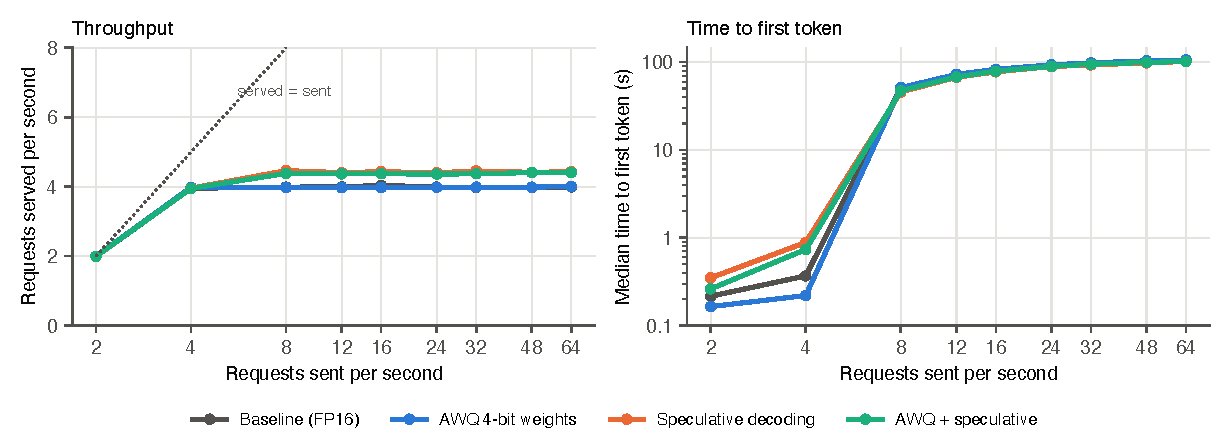
\includegraphics[width=\linewidth]{saturation.pdf}
\end{center}

Up to 4 requests/s, every request is served and the median TTFT stays between 0.16 and 0.9 s. Above that, the server finishes 4.0--4.4 requests/s regardless of how many are sent. The rest wait in the queue, and the median TTFT reaches 50--106 s.

None of the techniques moves this limit much. At 4 requests/s the GPU processes about 4,000 prompt tokens/s, so we think the limit is prefill compute. This still has to be confirmed by profiling. Everything above 4 requests/s is an overloaded server, and the latency numbers there are mostly queueing time.

\subsection{Below the limit}

\begin{center}
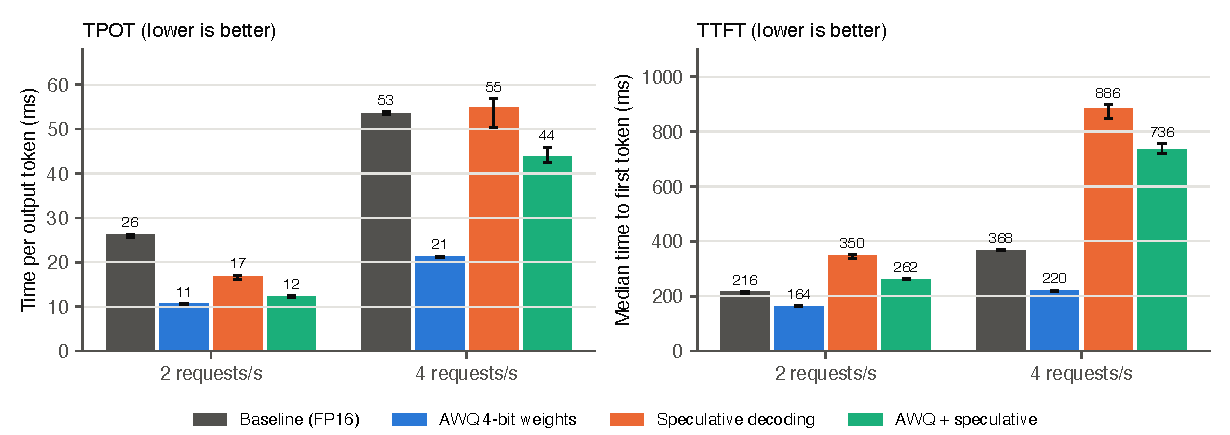
\includegraphics[width=\linewidth]{low_load.pdf}
\end{center}

Bars show the median of 4--6 runs, and the error bars show the range.

\textbf{AWQ} lowers TPOT about 2.5 times, from 26 to 11 ms at 2 requests/s and from 53 to 21 ms at 4 requests/s. TTFT is also lower at both loads. This matches decode being limited by memory bandwidth, since the AWQ model reads about a third as much weight data per token.

\textbf{Speculative decoding} lowers TPOT 1.6 times at 2 requests/s, but gives no gain at 4 requests/s. TTFT is higher at both loads, because the draft model also has to run prefill on the prompt.

\subsection{Contribution of each technique}

The table shows TPOT speed-up over the baseline, with the change in TTFT in brackets. The last column shows requests served per second when the server is overloaded.

\begin{center}
\begin{tabular}{@{}lccc@{}}
\toprule
Configuration & 2 requests/s & 4 requests/s & Overloaded, 16--64/s\\
\midrule
Baseline (FP16, vLLM defaults) & 1.00$\times$ & 1.00$\times$ & 4.0\\
\textbf{AWQ} & \textbf{2.47$\times$} ($-$24\%) & \textbf{2.52$\times$} ($-$40\%) & 4.0\\
Speculative decoding & 1.56$\times$ ($+$62\%) & 0.98$\times$ ($+$141\%) & \textbf{4.4}\\
AWQ + speculative decoding & 2.11$\times$ ($+$21\%) & 1.22$\times$ ($+$100\%) & 4.4\\
\bottomrule
\end{tabular}
\end{center}

Combining the two does not add the gains: AWQ alone (2.5$\times$) is faster than AWQ with speculative decoding (2.1$\times$ and 1.2$\times$). With AWQ, each pass of the 3B model is already cheap, while the draft model is not quantised and still runs 5 steps per round. About 55\% of the drafted tokens are accepted, i.e.\ around 3.7 tokens per verification pass, and this is no longer enough to pay for the draft steps.

Speculative decoding stops paying between 2 and 4 requests/s. At light load the GPU has idle compute during decode, which the draft model uses. At higher load the other requests in the batch already keep the GPU busy, so drafting and verification compete with them.

When overloaded, speculative decoding serves about 11\% more requests per second (4.4 vs.\ 4.0). However, TTFT is over a minute in every configuration at that point, so this gain is of little use in practice. AWQ gives no throughput gain when overloaded. This fits a prefill limit, because AWQ reduces the weight data read per pass but not the compute.

\section{Status}

\begin{tabularx}{\linewidth}{@{}P{3.6cm}P{2.4cm}X@{}}
\toprule
Item & Status & Note\\
\midrule
M1: AWQ & Done & 2.5$\times$ lower TPOT below 4 requests/s; output quality not yet measured\\
M1: FP8 KV cache & Blocked & Needs the CUDA toolkit on the server\\
M1: batching & Not started & Single GPU, so the choice is batch size and scheduling, not sharding\\
M2: speculative decoding & Done & Break-even between 2 and 4 requests/s\\
M2: prefix caching & Next & Needs prompts with shared prefixes\\
M3: contribution of each technique & First version & One prompt length only\\
\bottomrule
\end{tabularx}

\section{Limitations and next steps}

\begin{itemize}
\item All runs use one prompt length (1,024 tokens) and prompts with no shared prefix.
\item The load generator sends requests at a fixed rate, so loads above the limit only measure queueing.
\item AWQ output quality is not measured yet.
\item One GPU and one model size.
\end{itemize}

\begin{tabularx}{\linewidth}{@{}XXX@{}}
\toprule
Next two weeks & Then & Before the final review\\
\midrule
Prompt lengths 512--6,144 & Fixed-concurrency sweep & Contribution of each technique across regimes\\
Prefix caching off vs.\ on, with shared prefixes & 2--3 draft tokens; other draft methods & Best setup per regime\\
CUDA toolkit; FP8 KV cache & Goodput at the latency target & Profiling of the limit\\
AWQ quality on a small benchmark & Batch-size and scheduling tuning & Final plots and scripts\\
\bottomrule
\end{tabularx}

For M1 we use TTFT under 1 s and TPOT under 50 ms as the latency target, and will report goodput: the requests per second that meet both.

\section{Repository}

\url{https://github.com/anupchavan/efficient-llm-serving} contains the benchmark script (\texttt{scripts/}), the 201 raw result files (\texttt{data/raw/}), a per-run summary table (\texttt{data/summary.csv}), the analysis and plotting scripts (\texttt{analysis/}), the figures, this report and the slides.

\section*{References}
\begin{enumerate}[label={[\arabic*]},leftmargin=2em]
\item Efficient Memory Management for Large Language Model Serving with PagedAttention --- Kwon et al., SOSP 2023. \url{https://arxiv.org/abs/2309.06180}
\item Taming Throughput-Latency Tradeoff in LLM Inference with Sarathi-Serve --- Agrawal et al., OSDI 2024. \url{https://arxiv.org/abs/2403.02310}
\item SGLang: Efficient Execution of Structured Language Model Programs --- Zheng et al., NeurIPS 2024. \url{https://arxiv.org/abs/2312.07104}
\item Fast Inference from Transformers via Speculative Decoding --- Leviathan et al., ICML 2023. \url{https://arxiv.org/abs/2211.17192}
\item AWQ: Activation-aware Weight Quantization for LLM Compression and Acceleration --- Lin et al., MLSys 2024. \url{https://arxiv.org/abs/2306.00978}
\end{enumerate}

\end{document}
